\subsubsubsection{Scheduling}
The scheduling package contains all the logic needed to have worker threads
which consume work items, which correspond to the actions that occur in our
simulations.

The scheduling system instantiates two executors, one for the travellers and
one for traffic lights: this is done to minimize time drifts among different
traffic lights (which can toggle their state smoother, without having to
compete with travellers to be dequeued and executed).
However, these two executors are the same package, just instantiated twice with
a different number of worker threads.

We will present our scheduling component by first describing how our system
starts, then how it executes work items and how it stops.
Finally, we will have a quick look at the \texttt{Callback} hierarachy.

\paragraph{Start}

Scheduling is started asynchronously by providing a list of work items
(or \textit{agenda}), which correspond to either travellers' or traffic
lights' actions.
Scheduling will just process this list, by registering events at the time
reported in the agenda.

\paragraph{Execution}

In Figure \ref{fig:schedule-execution} we show how a request to schedule an
entity is handled:

\begin{enumerate}
  \item First, the \texttt{Scheduler} delegates the execution of an action to
    an \texttt{Executor}: the latter is an interface which is implemented by
    \texttt{SimpleExecutor} in our system;
  \item \texttt{SimpleExecutor} registrates a timer to defer the action;
  \item When the timer expires, it asks to its \texttt{Executor} reference to
    execute an action (the one which originally had to be scheduled);
  \item If it is not stopped, \texttt{SimpleExecutor} add this action to the
    \texttt{WorkQueue};
  \item At this point, an idle \texttt{WorkerThread} which was for an item to
    execute can fetch the new item\footnote{if the queue was empty, otherwise
    items are enqueued with FIFO priority} and consume it.
\end{enumerate}

\begin{figure}[H]
\centering
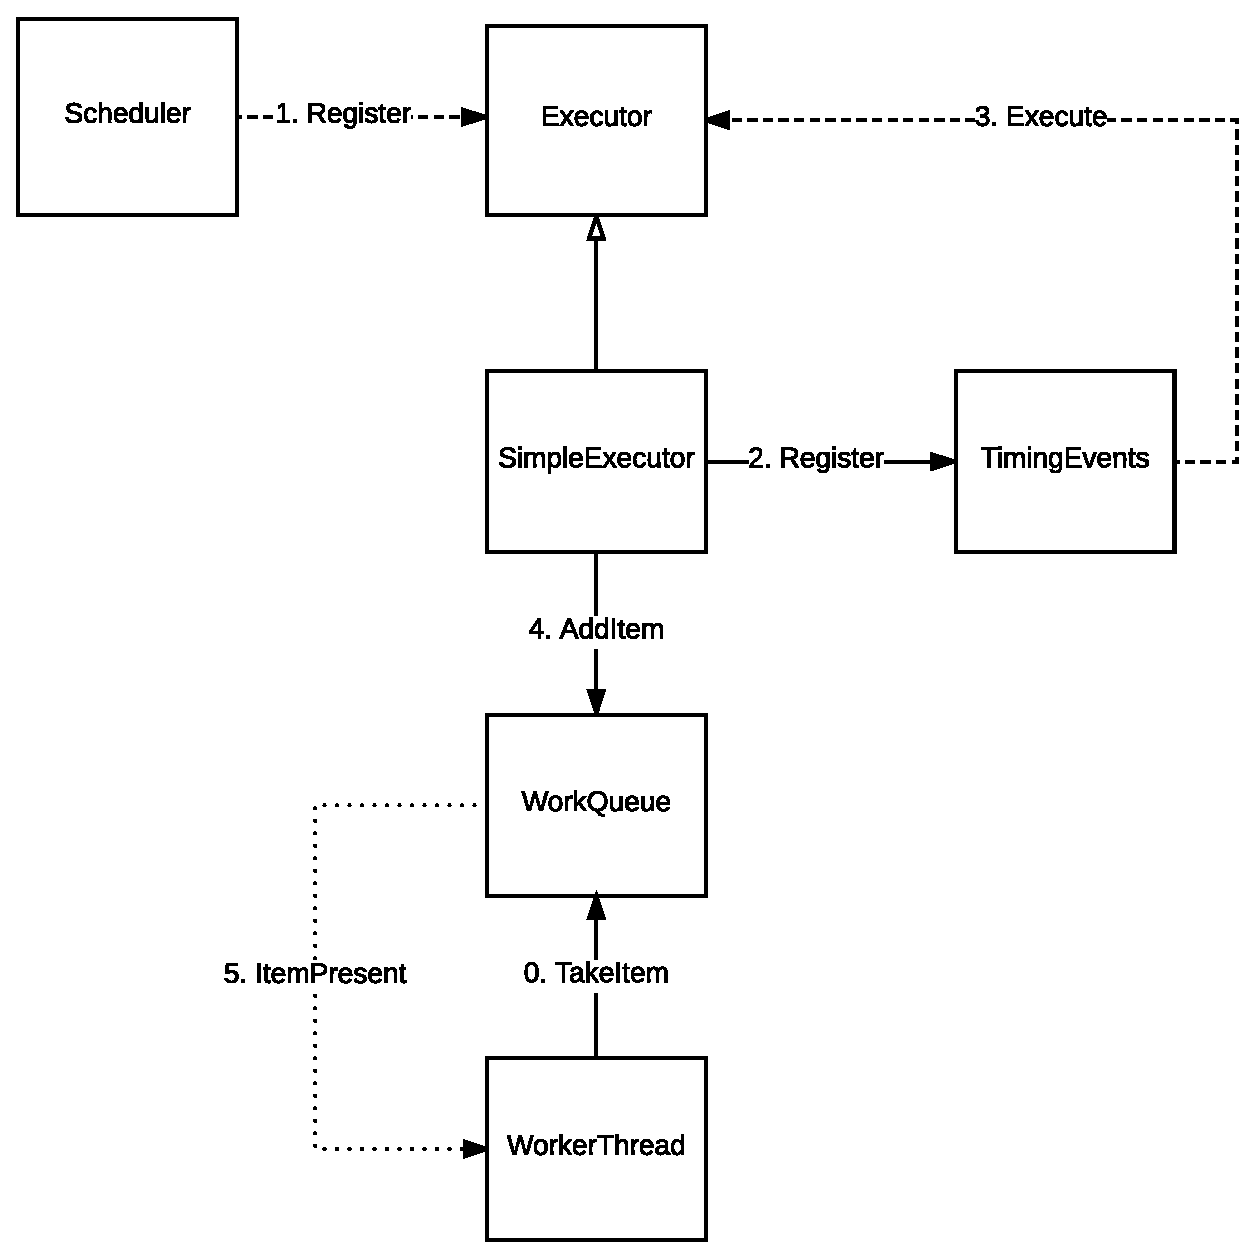
\includegraphics[scale=0.5,keepaspectratio]{images/solution/app/backend/scheduling-execution.eps}
\caption{Execution of a work item}
\label{fig:schedule-execution}
\end{figure}

\paragraph{Termination}

In Figure \ref{fig:schedule-termination} we show how a request to schedule an
entity is handled:

\begin{enumerate}
  \item First, the \texttt{Scheduler} asks the \texttt{Executor}s to shutdown;
  \item \texttt{SimpleExecutor} stops itself and then loads, in the work queue,
    as many poison pills as many linked worker threads;
  \item Eventually each worker thread will fetch a poison pill from the work
    queue;
  \item When trying to consume a poison pill, a worker thread will stop
    itself and will notify a proxy between it and the Executor;
  \item Finally, when all the workers are stopped, the Executor is unblocked
    from the synchronous entry provided by the Proxy.
\end{enumerate}

\begin{figure}[H]
\centering
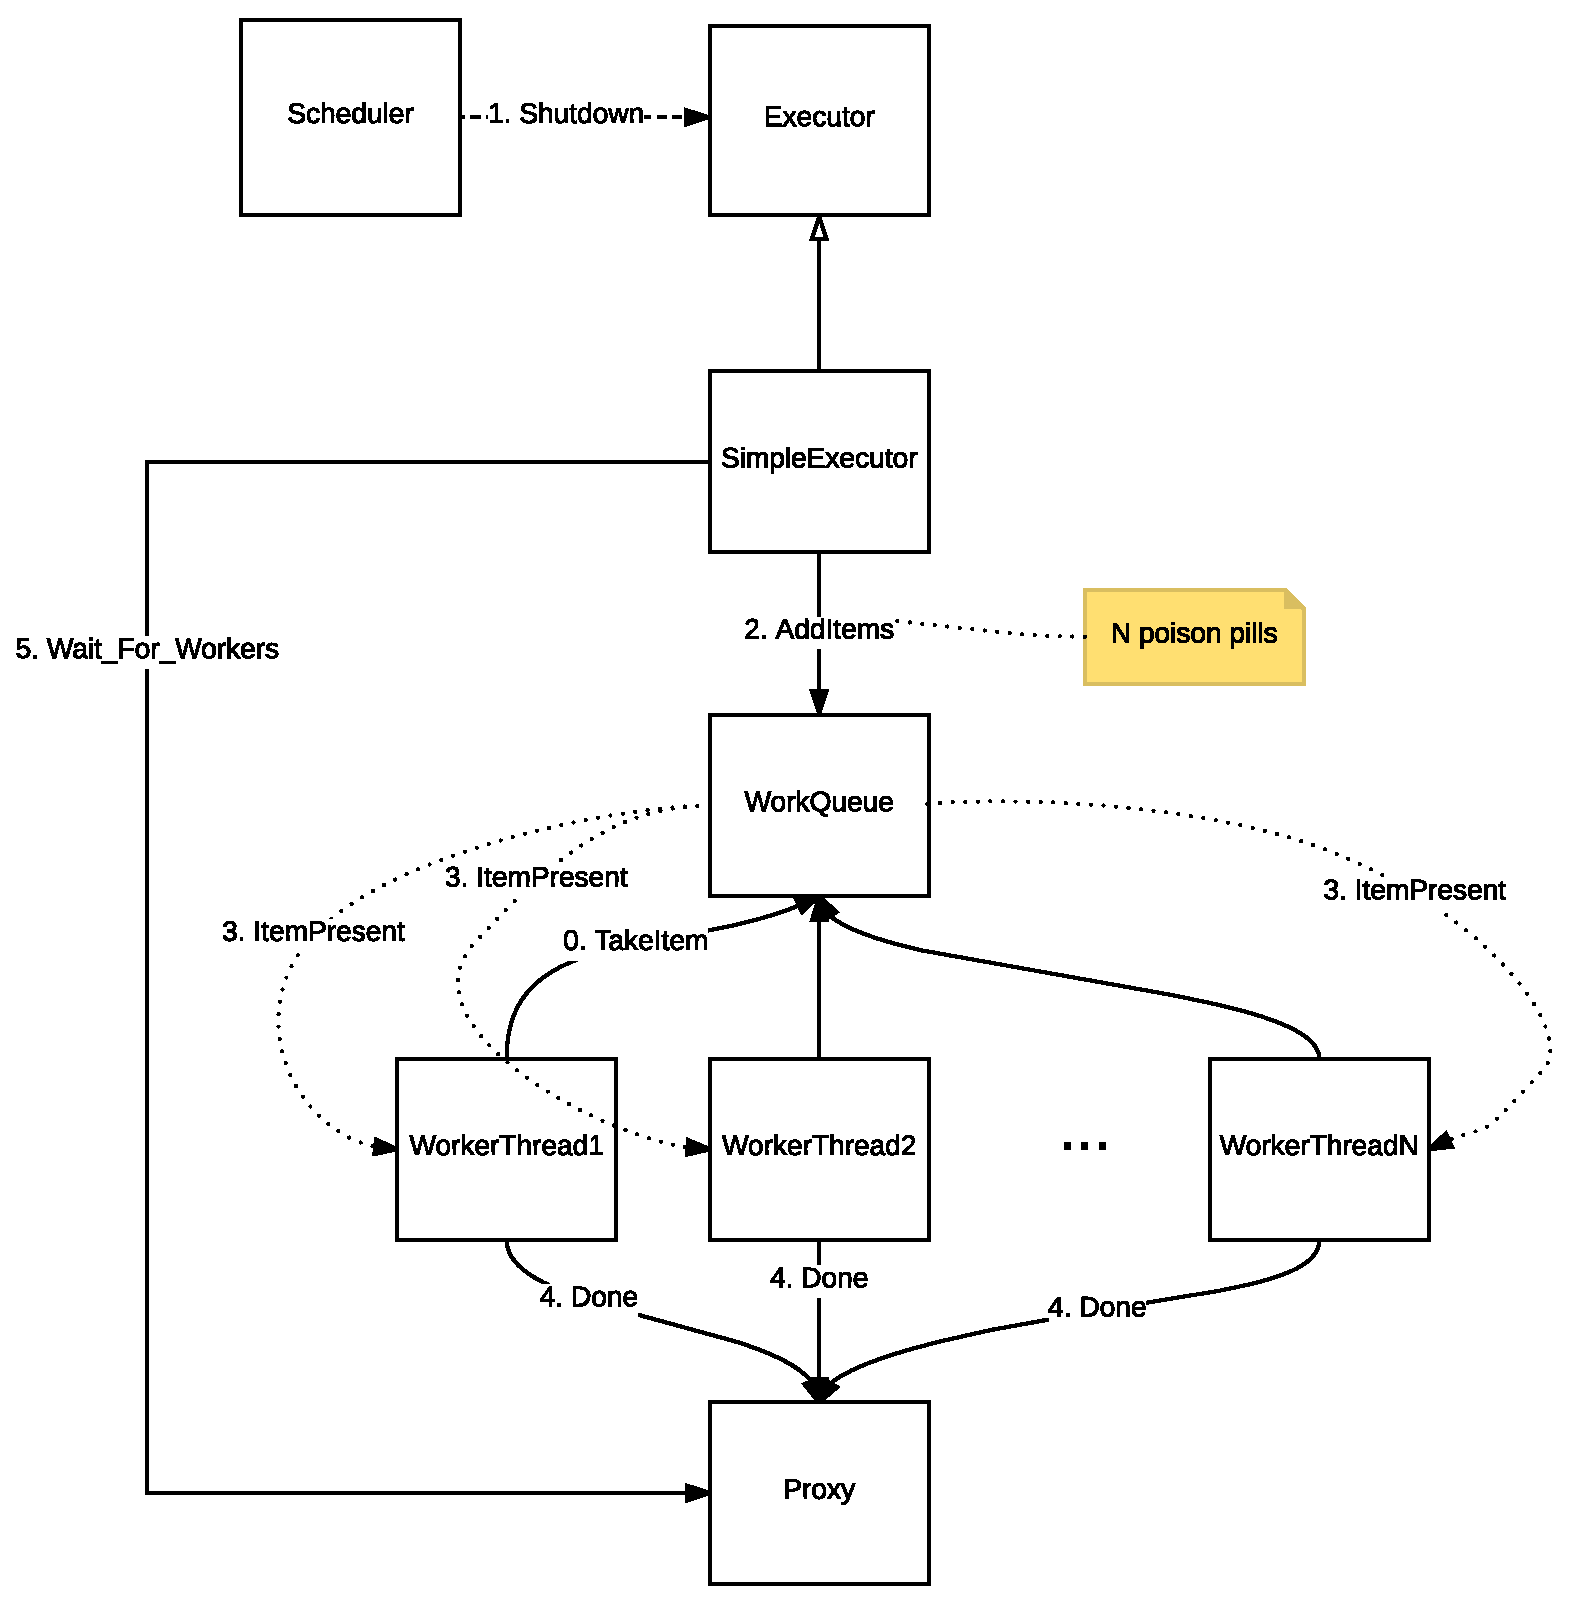
\includegraphics[scale=0.5,keepaspectratio]{images/solution/app/backend/scheduling-termination.eps}
\caption{Scheduling termination}
\label{fig:schedule-termination}
\end{figure}

\paragraph{Callbacks}

As we can see from the code, we implemented four callbacks (actually, two
pairs of success/failure callbacks).
We felt the necessity to introduce this mechanism in our system to avoid
blocking on synchronous remote calls.
In fact, if we chose to block on synchronous calls, there could be an item in
the work queue awaiting to be executed with all the worker threads currently
blocked on several remote calls.

It is glaring that this behaviour would sensibly harm concurrency: therefore we
decided to separate the blocking part of a remote call and the actions to take
in response to a given outcome for it, like the NodeJS runtime does.
We bound these pairs of callbacks to an asynchronous queue triggered by network
interruptions, thus being able to free the worker thread and minimizing the
blocking overhead.
% TODO: Retry transmission?
